\documentclass{article}

% Language setting
% Replace `english' with e.g. `spanish' to change the document language
\usepackage[english]{babel}

% Set page size and margins
% Replace `letterpaper' with `a4paper' for UK/EU standard size
\usepackage[letterpaper,top=2cm,bottom=2cm,left=3cm,right=3cm,marginparwidth=1.75cm]{geometry}

% Useful packages
\usepackage{amsmath}
\usepackage{amssymb}
\usepackage{graphicx}
\usepackage{inconsolata}
\usepackage{minted}
\usepackage[colorlinks=true, allcolors=blue]{hyperref}

\title{Innleveing 1}

\begin{document}
\maketitle

\section{Oppgave 1}

\subsection{a) Hva kjennetegner en god hypotese?}

B. Den er falsifiserbar

\subsection{b) Hva er hovedpoenget med den hypotetisk deduktive metoden?}

C. Å teste hypotesen eksperimentelt og eventuelt endre dem

\subsection{c) Du før oppgitt $v= 3,40 m/s$. Hva er måtallet her?}

C. m/s

\subsection{d) Du før oppgitt $v= 3,40 m/s$. Hva er størrelsen her?}

A. 3,40

\subsection{e) Du før oppgitt $v= 3,40 m/s$. Hvor mange gjeldene siffer har vi her?}

B. 2

\subsection{f) Hvilken av følgene størrelser har to gjeldene siffer?}

A. A, C og D

\subsection{g) En bil kjører med konstant fart. Den bruker $2.25s$ på å kjøre $10 m$. Hva er farten?}

D. $4 m/s$

\section{Oppgave 2}

\subsection{a) Hvilken type graf er det?}

C. Akselerasjonsgraf

\subsection{b) Hva er farten til bilen når tiden starter?}

B. $4 m/s$

\subsection{c) Hvor langt kjører bilden de første 5 sekundene?}

C. $45 m$

\subsection{d) Hva er akselerasjonen til bilen?}

D) $2 m/s^2$

\subsection{e) Hvilken er grafene under kan være strekningsgrafen til bilen?}

C kan være det

\subsection{f) hva er farten til bilen?}

D. $v(t) = 3 - 4t$

\section{Oppgave 3}

\subsection{a) Hva er bevegelsesmengden til den grønne klossen?}

B. $p = 5kg \cdot 3 m/s = 15 kg \cdot m/s$

\subsection{b) Hvilken type støt er det mellom de to kassene?}

C). Uelastisk

\subsection{c) Er det rimelig å anta at bevegelsesmengden er bevart i støtet?}

B. Ja, bevegelsesmengden er alltid bevart

\subsection{d) Vi antar at bevegelsesmengden er bevart. Hva er den samlede bevegelsesmengden til klossene etter støtet?}

C) $14 kg \cdot m/s$

\subsection{e) Hvilken retning beveger klossene seg etter støttet?}

C. Mot høyre

\subsection{f) Er det rimelig å anta at den kinetiske enerigen er bevart i støtet?}

A. Ja kinetisk energi er alltid bevart i støt

\subsection{g) Hvor stort er implusen på den grønne klossen i støtet?}

A. Lik endringen i bevegelsesmenge for den grønne klossen

\section{Oppgave 4}

\subsection{a) Hvor høy kommer ballen?}

Jeg finner høyden ved å sette fartsfunksjonen lik 0

$v(t) = 8.5 - 9.81 t = 0 \rightarrow t = 0.87$

Så setter $t$ i strekningsfunksjonen

$s(t) = \int v(t)$

$s(0.87) = 3.68$

Ballen får en høyde på $3.68m$

\subsection{b) Hvor lang tid bruker ballen på å komme til det øverste punktet i banen sin?}

Basert på det jeg fant ut i oppgave a bruker den ca $0.87s$

\subsection{c) Hvor lang tid bruker ballen fra den kastes og til den er tilbake ved Maries hånd?}

For å finne tiden setter jeg strekningsfunksjonen lik 0

$s(t) = \int v(t) = -4.91 t^2 + 8.5t + 0$

$s(t) = 0 \rightarrow t = 0 \lor t = 1.73s$

Ballen bruker $1.73s$

\subsection{d) Hva er farten til ballen i det den passerer Maries hånd på vei ned?}

$v(1.73) = -8.47$

Farten er $8.47 m/s$ mot bakken

\subsection{e)} Ballen lander på bakken nedfor verandaen etter 2,12 sekunder etter kastet. Hvor høyt over bakken kastet Marie ballen fra?

Setter 2,12 i strekningsfunksjonen

$s(2,12) = -4.03$

Marie kastet ballen 4.03 meter over bakken

\subsection{f) Tegn en fartsgraf for ballen}

\begin{figure}[H]
    \centering
    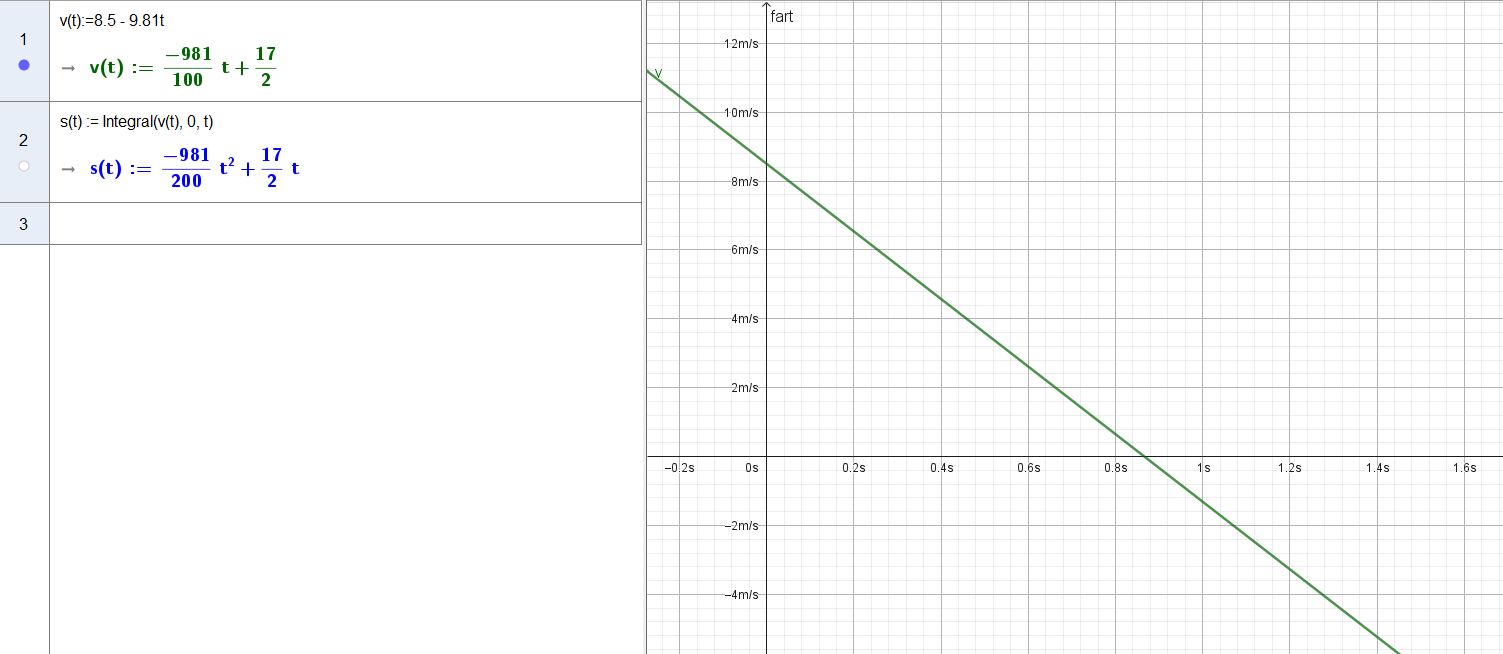
\includegraphics[width=0.7\textwidth]{bilder/opg4f.png}
    \caption{Fartsgrafen}
\end{figure}

\subsection{g) Tegn en akselerasjonsgraf for ballen}

\begin{figure}[H]
    \centering
    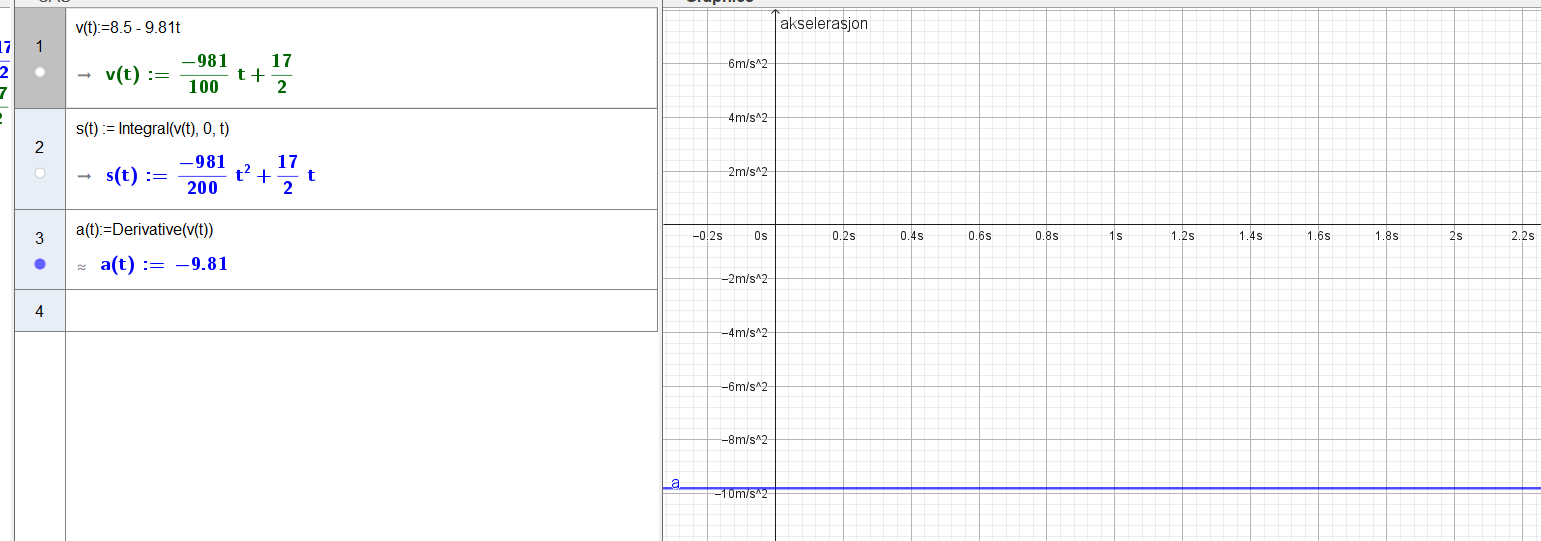
\includegraphics[width=0.7\textwidth]{bilder/opg4g.png}
    \caption{Akselerasjonsgrafen}
\end{figure}

\subsection{h) Hva er den potensielle energien til ballen når den er toppunktet av kastebanen?}

potensiell energi er: $E_p = mgh$

$E_p = 0.150 kg \cdot 5,00 m \cdot 9.81 m/s^2 = 7.36 J$

Den potensielle er $7.36$ Joule

\subsection{i) Hva er den kinetiske energien til ballen akkurat i det forlater hånden hennes?}

Jeg vet at den mekaniske energien er bevart. Derfor er den kinetiske energien lik den potensielle energien fra toppunktet av kastebanen fra hånden hennes

Den kinetiske energien er $7.36$ Joule

\subsection{j)}

Kinetisk energi er $E_k = \frac{1}{2} m v^2$

Da er farten: $\sqrt{\frac{2E_k}{m}} = v$

$\sqrt{\frac{2 \cdot 7.36 J}{0.150 kg}} = 9.91 m/s$

ballen hadde en fart på $9.81 m/s$ når den forlot hånden hennes

\subsection{k)}

Marie gjør er arbeid på $7.36J$ på ballen

\subsection{m)}

\begin{figure}[H]
    \centering
    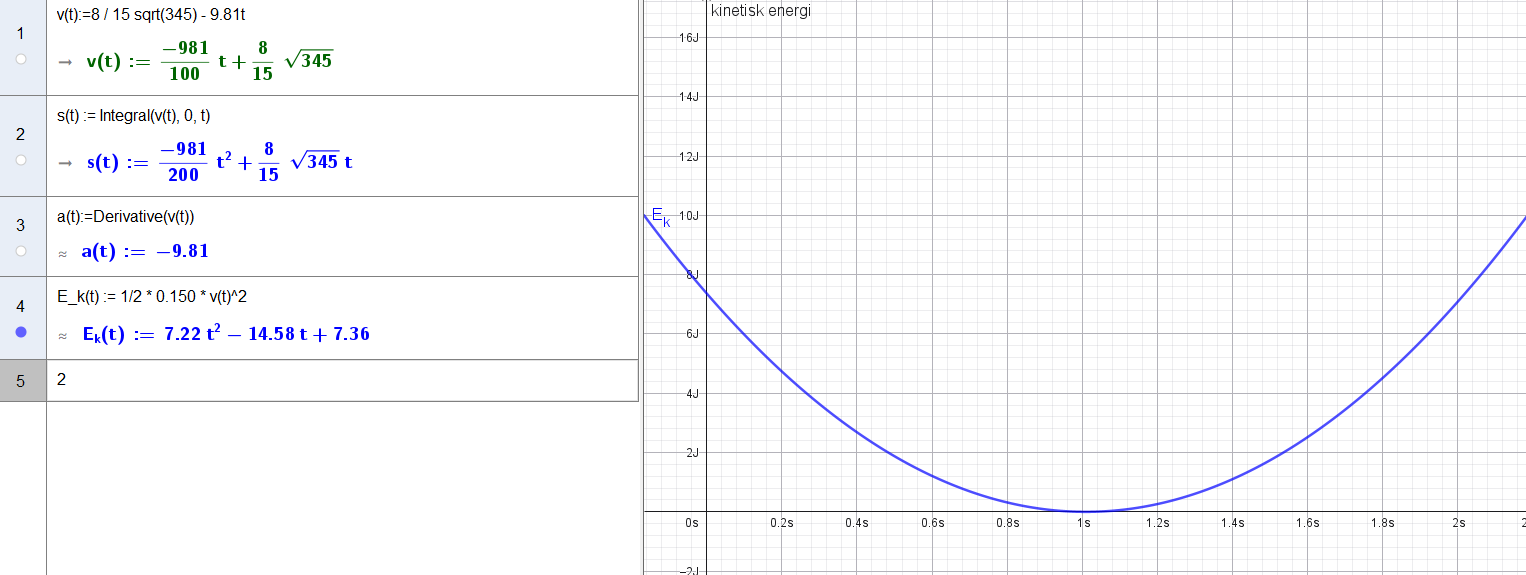
\includegraphics[width=0.7\textwidth]{bilder/opg4m.png}
    \caption{Kinetisk energi}
\end{figure}

\subsection{n)}

\begin{figure}[H]
    \centering
    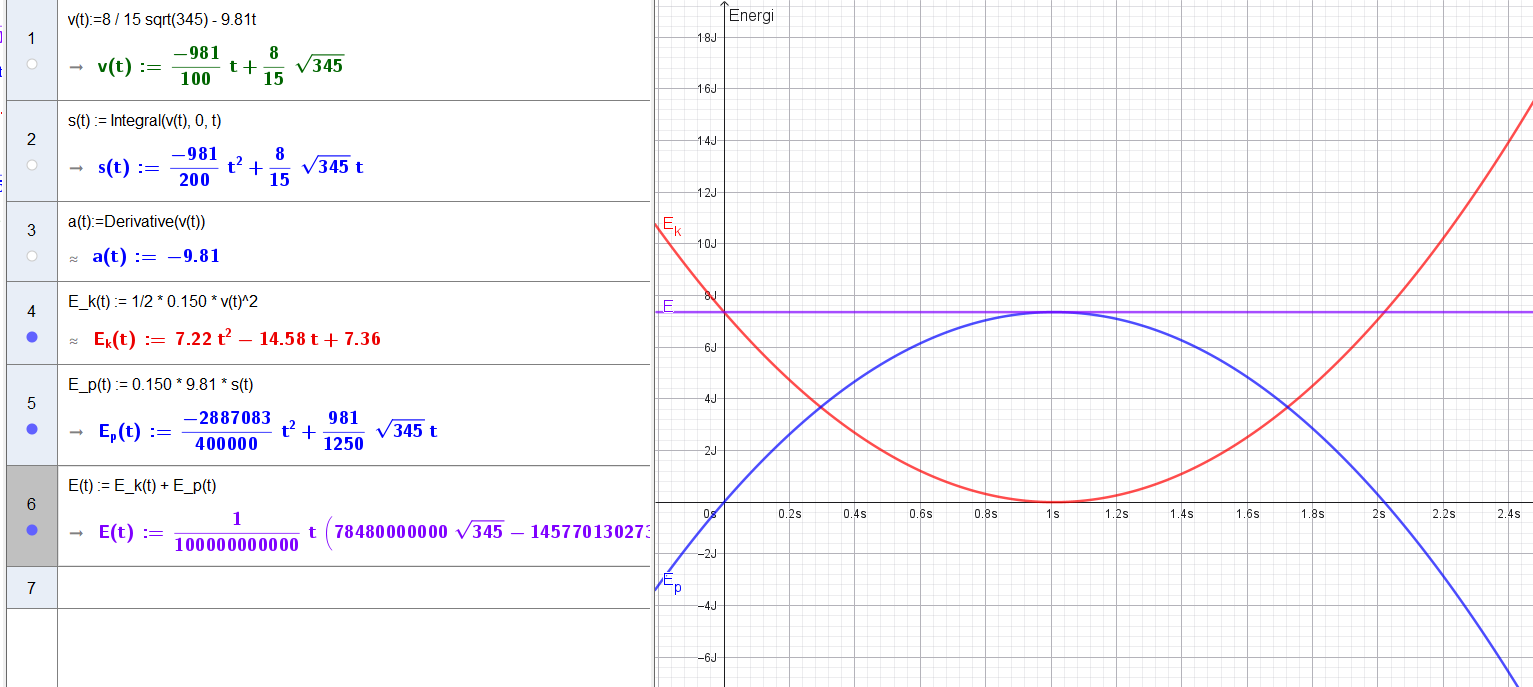
\includegraphics[width=0.7\textwidth]{bilder/opg4n.png}
    \caption{Energi}
\end{figure}

\subsection{o)}

Regner ny potensiell energi: $4,00 m \cdot 0.150 kg \cdot 9.81 m/s^2 = 5.89 J$

Luftmotsanden er differansen mellom ballen med og uten Luftmotsanden

$7.36 J - 5.89 J = 1.47J$

Luftmotsanden har gjort er arbeid på $1.47 J$

\section{Oppgave 5}

\subsection{a)}

\begin{figure}[H]
    \centering
    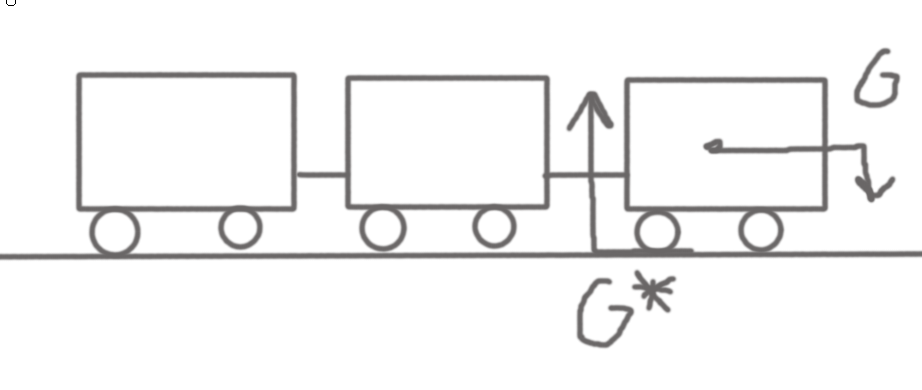
\includegraphics[width=0.7\textwidth]{bilder/opg5a.png}
    \caption{Toget står stille}
\end{figure}

\subsection{b)}

\begin{figure}[H]
    \centering
    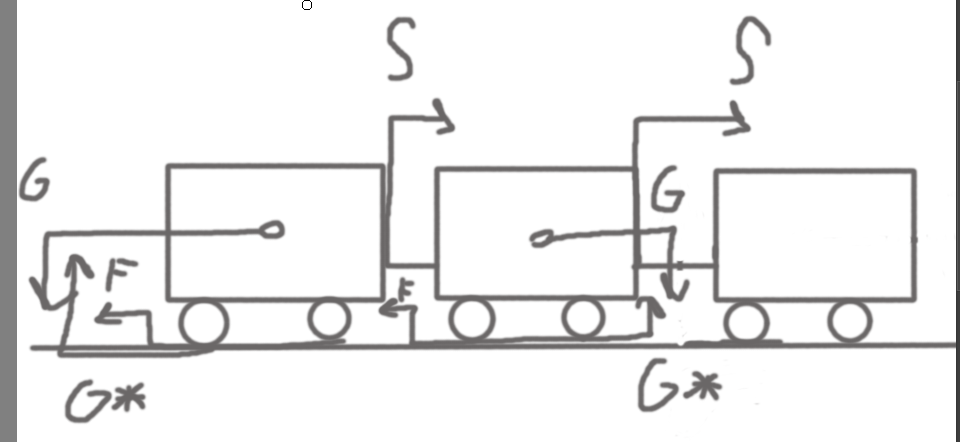
\includegraphics[width=0.7\textwidth]{bilder/opg5b.png}
    \caption{Toget beveger seg}
\end{figure}

\subsection{c)}

Regner lekelokmotivet med voknene som et system. Få får den en masse på $0,500 kg$



\bibliographystyle{alpha}
\bibliography{sample}

\end{document}
